\documentclass[9pt,twocolumn]{extarticle}

\usepackage[hmargin=0.5in,tmargin=0.5in]{geometry}
\usepackage{amsmath,amssymb}
\usepackage{times}
\usepackage{graphicx}
\usepackage{subfigure}

\usepackage{cleveref}
\usepackage{color}
\newcommand{\TODO}[1]{\textcolor{red}{#1}}

\newcommand{\FPP}[2]{\frac{\partial #1}{\partial #2}}
\newcommand{\argmin}{\operatornamewithlimits{arg\ min}}
\author{Siwang Li}

\title{Full Space Material Fitting}

%% document begin here
\begin{document}
\maketitle

\setlength{\parskip}{0.5ex}

\section{Introduction}
\paragraph{Formulation.} Given the optimized modal basis $W$, the corresponding eigenvalues
$\Lambda$, and the mass matrix $\tilde{M}$, we solve for the Shear modulus
$G=(G_1,\cdots,G_{tet})$, Lame's first parameter $l=(l_1,\cdots,l_{tet})$ for
all tetrahedrons. Currently, I have tried several methods to solve this problem,
all of which have the similar formulation
\begin{equation} \label{all}
  \min_{G,l}(\phi_e(G,l)+\mu_{g}\phi_s(G)+\mu_{l}\phi_s(l)), \mbox{s.t. } G_i>0, l_i>0
\end{equation}
where $\mu_g, \mu_l$ are some penalty parameters, and
\begin{equation} \label{smooth}
  \phi_s(x) = \frac{1}{2}\sum_{(i,j)_{n}}(x_i-x_j)^2V_{i,j}, \mbox{ for all
    tet. }i
\end{equation}
which indicates that, the material $x$ should be smooth, where $(i,j)_{n}$ represents a
neighbor tetrahedron pair, and $V_{i,j}=\frac{1}{4}(v_i+v_j)$ with $v_i$ is the
volume of tetrahedron $i$. 

\paragraph{Experiments.} There are different methods to define
$\phi_e(G,l)$. For each method, two experiments are used to check the results,
and a same model with two different materials are used in all experiments as
shown in figure \ref{ref_E}. In the first experiment, we compute $W$ and
$\Lambda$ using the reference material as shown in figure \ref{ref_E}, then we
use $W$ and $\Lambda$ to solve eq. (\ref{all}) to obtain $G,l$ to check the
methods. In the second experiment, we use the material in figure \ref{ref_E} to
produce an animation sequence, then use this animation sequence and uniform
material as input to our material optimization system to generate the optimal
basis $W=\hat{W}S$ and $\Lambda$, which are adopted as input in eq. (\ref{all})
to obtain $G,l$. We will convert $G$ and $l$ to obtain the Young's $E$ and
Poisson's ration $v$, which are presented as the resulting material.

\paragraph{Constrained nodes.}
In all the experiments, the left end of the beam is fixed, and for these
constrained nodes, we first remove the corresponding columns and rows from
$\tilde{K}, \tilde{M}, M$, and remove the corresponding rows in $W$, then use
them to solve for $G,l$ and maybe $\rho$.

\paragraph{Summary.}
All the methods produce reasonable results in the first experiment, however,
no good results are obtained for the second experiment. I have also tried to
use NNLS and IPOPT to solve these problems respectively, and the results of
IPOPT seems better than NNLS. I suppose that this is because the hessian of this
problem is ill-conditional, and IPOPT is more robust in solving such problem. In
the following, I will introduce different methods to define $\Phi_e$ and present
the corresponding results.

\begin{figure}
  \centering
  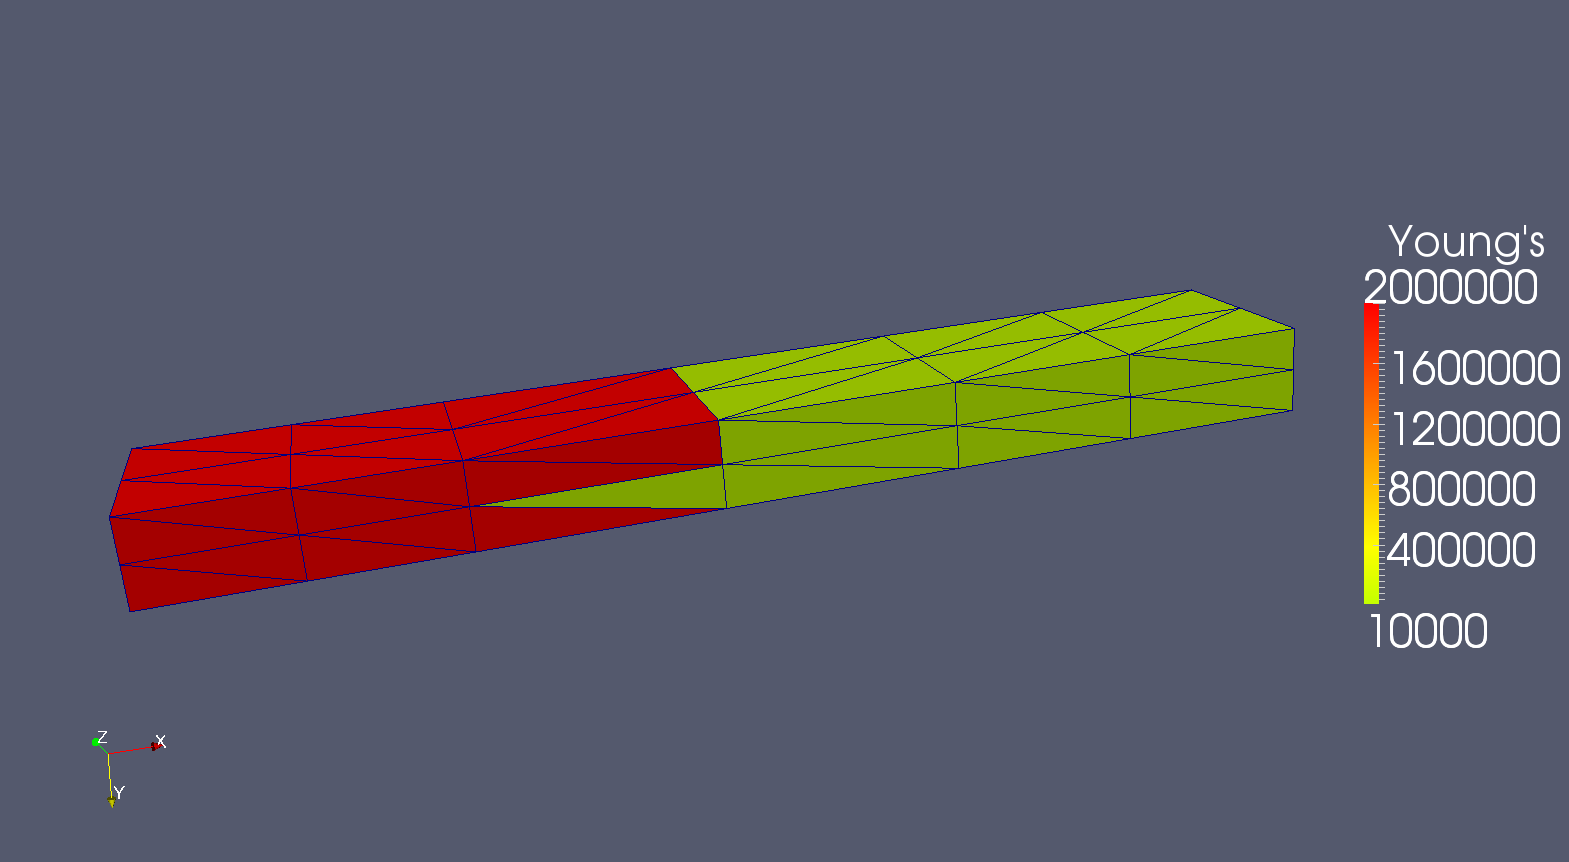
\includegraphics[width=0.42\textwidth]{./figures/ref_E.png}
  \caption{The reference material distribution for all the experiments. The
    density and Poisson's ratio are uniform, which are $1000 kg/m^3$ and $0.45$
    respectively.}
  \label{ref_E} 
\end{figure}

\section{Based on modal analysis}\label{sec:based-modal-analysis}
We assume that the desired $G,l$ should make sure that the given $W$ and
$\Lambda$ can satisfy the modal analysis equation, thus we define
\begin{equation} \label{ma}
  \phi_e(G,l) = \frac{1}{2}\|K(G,l)W-\tilde{M}W\Lambda\|_2^2
\end{equation}
The results are shown in figure \ref{fig:ma}. The results of the first
experiment is exactly equal to the ground truth material. However, when $\mu_g$
and $\mu_l$ is small, we will get many zeros in $G$ and $\rho$, and get wrong
elastic material (not presented here). While when these parameters are large (we
use $\mu_g=\mu_l=1000$ here), the results will also be far from the reference
material, though the we assume that the mass matrix $\tilde{M}$ is already given
here.
\begin{figure}[htb]
  \centering
  \newcommand{\Pic}[1]{
    \includegraphics[width=0.2\textwidth]{./figures/ma-#1.png}}
  \begin{tabular}{@{}cc@{}}
    \Pic{cv}&\Pic{ov}\\
    \Pic{ce}&\Pic{oe}\\
    First Exp. &Second Exp. 
  \end{tabular}\vspace*{-3mm}
  \caption{Results for the method based on modal analysis. We use $r=4,
    \mu_g=\mu_l=10^{-15}$ for the first experiment, and use $r=4,
    \mu_g=\mu_l=1000$ for the second experiment. Here $r$ is the number of
    columns in $W$.}
  \label{fig:ma}
\end{figure}

\section{Based on diagonalization}
We assume that the desired $G,l$ should make sure that the given $W$ can
diagonalize $K(G,l)$ to obtain $\Lambda$, and thus we define
\begin{equation} \label{diag}
  \phi_e(G,l) = \frac{1}{2}\|W^TK(G,l)W-\Lambda\|_2^2
\end{equation}
The results are shown in figure \ref{fig:diag}. The results for the first
experiment is not as good as the results of section
\ref{sec:based-modal-analysis}, and the results of the second experiment are
better than section \ref{sec:based-modal-analysis}. However, the given mass
matrix $\tilde{M}$ have not been adopted in this method, and the amplitude of
$G$ and $l$ are far from the desired reference material.
\begin{figure}[htb]
  \centering
  \newcommand{\Pic}[1]{
    \includegraphics[width=0.2\textwidth]{./figures/diagk-#1.png}}
  \begin{tabular}{@{}cc@{}}
    \Pic{cv}&\Pic{ov}\\
    \Pic{ce}&\Pic{oe}\\
    First Exp. &Second Exp. 
  \end{tabular}\vspace*{-3mm}
  \caption{Results for the method based on diagonalization. We use $r=4,
    \mu_g=\mu_l=10^{-15}$ for both experiments. }
  \label{fig:diag}
\end{figure}


\section{Diagonalization with given mass matrix}
This formulation is designed with the assumption that the following motion
equation can be diagonalized by some basis matrix $\tilde{W}$,
\begin{equation} \label{motion_eq}
  \tilde{M}\ddot{x} + K(G,l)x = 0
\end{equation}
where $\tilde{M}$ is the given mass matrix. To achieve this, we first solve for
the density $\rho$ using 
\begin{equation} \label{mass}
   \min_{\rho}\frac{1}{2}\|W^TM(\rho)W-I\|_2^2+\mu_{r}\phi_s(\rho), \mbox{s.t. }
   \rho_i>0
\end{equation}
Then transform the basis matrix $W$ as
\begin{equation} \label{W_ext}
  \tilde{W}=\tilde{M}^{-\frac{1}{2}}M^{\frac{1}{2}}W
\end{equation}
It is obviously that $\tilde{W}^T\tilde{M}\tilde{W}\approx I$, and we can solve $G,l$
by using
\begin{equation} \label{diag_k}
  \phi_e(G,l) = \frac{1}{2}\|\tilde{W}^TK(G,l)\tilde{W}-\Lambda\|_2^2
\end{equation}
The results are shown in figure \ref{fig:diag_k}. For the second experiment, we
need to use a large $\mu_m$ here, as when $\mu_m$ is small, there will be a lot
of zeros in the resulting $\rho$, and we can not compute $M^{-\frac{1}{2}}$.
\begin{figure}[htb]
  \centering
  \newcommand{\Pic}[1]{
    \includegraphics[width=0.2\textwidth]{./figures/diag-fix-m-#1.png}}
  \begin{tabular}{@{}cc@{}}
    \Pic{cv}&\Pic{ov}\\
    \Pic{ce}&\Pic{oe}\\
    First Exp. &Second Exp. 
  \end{tabular}\vspace*{-3mm}
  \caption{Results for the method based on diagonalization with given mass
    matrix. We use $r=10, \mu_m=\mu_g=\mu_l=10^{-15}$ for the first experiment,
    and use $r=4, \mu_m=1000, \mu_g=\mu_l=10^{-15}$ for the second experiment.}
  \label{fig:diag_k}
\end{figure}

% \section{Multiply the inverse mass matrix}
% In this formulation, we define
% \begin{equation} \label{diag}
%   \phi_e(G,l) = \frac{1}{2}\|W^TM^{-1}K(G,l)W-\Lambda\|_2^2
% \end{equation}
% Though this method produce much better results than the above methods, the
% resulting motion equation in full space may not be diagonalized by $W$, and thus
% this definition is not correct. The results are shown in figure \ref{fig:inv_m}.
% \begin{figure}[htb]
%   \centering
%   \newcommand{\Pic}[1]{
%     \includegraphics[width=0.2\textwidth]{./figures/ma-#1.png}}
%   \begin{tabular}{@{}cc@{}}
%     \Pic{cv}&\Pic{ov}\\
%     \Pic{ce}&\Pic{oe}\\
%     First Exp. &Second Exp. 
%   \end{tabular}\vspace*{-3mm}
%   \caption{Results for the method based on modal analysis.}
%   \label{fig:inv_m}
% \end{figure}


\end{document}